\section{Evaluation}

Recently, Haehn et al. discussed requirements for interactive proofreading software and evaluated three different existing tools on connectomics data \cite{haehn_dojo_2014}. The authors performed a non-expert user study and stated that their software Dojo provides better results than other tools due to a minimalistic user interface and sophisticated 3D volume rendering. We use their findings as baseline for the evaluation of our method and compare \textit{fully automatic proofreading} versus \textit{user-guided proofreading} versus \textit{interactive proofreading}. For comparison, we use the same data as Haehn et al. which is as well as the user generated proofreading results, publicly available. The data is part of the ISBI 2013 challenge dataset (1024x1024x100 pixels) which was acquired using a serial section scanning electron microscope (ssSEM) with a resolution of 6x6x30nm/pixel. Haehn et al. perform their user study on the most representative sub-volume (400x400x10 pixels) in terms of distribution of object size. For optimal comparison, we use exactly the same data.

\textbf{Fully automatic proofreading.} During training, we defined parameters for our split and merge classifiers including thresholds for automatic correction of these. To evaluate automatic proofreading, we use both classifiers in a greedy fashion and choose the split and merge errors with the best scores for automatic correction.

\textbf{User-guided proofreading.} For the evaluation of user-guided proofreading, we simulate user feedback during our automatic correction from above by comparing the resulting segmentation before and after each performed correction. Since users are not perfect, we also introduce an error rate which simulates falsely specified user feedback.

\textbf{Interactive proofreading.} We use the published results from Haehn et al. to compare our results against fully interactive proofreading using their software Dojo. We studied the published results and gain additional insights, e.g. edits per time a user performs on average.

Each method is compared against the available manual segmentation of the data for similarity and is scored using the variation of information (VI) metric. VI is a measure of the distance between two clusterings, closely related to mutual information, but lower being better.






For evaluation, we 

Merge errors more seldom than split errors

ran evaluation on the last 5 slices from our data (ground truth and rhoana)
1024x1024: ~10 minutes per slice

ran evaluation on dojo study subvolume from a different dataset
~400 seconds for subvolume just split errors
threshold: merge error for p<.3, split error for p>.7




Paragraph: introduction of how (broadly) we evaluate the method. Where does the ground truth come from?

Equation: What is VI?

\subsection{Split error evaluation}

Paragraph: What is the process of evaluating split errors?

Paragraph: What do we compare against? What is the result? Why is the performance better?

\begin{table}[t]
\begin{tabular}{ll}
\toprule
Method & VI improvement after fixing split errors \\
\midrule
Jain design & \\
Jain design variation & \\
Our design &  \\
Our design variation & \\
\bottomrule
\end{tabular}
\caption{This is a table of results. It shows the comparison to Jain et al., and the comparison to different variations of these algorithms with the varying overlap regions.}
\label{tab:spliterrorcorrectionperformance}
\end{table}

\subsubsection{Analysis}

Paragraph: Demonstration of ROC curves for VI performance in split error adjustment as the threshold varies.

\begin{figure}[t]
\missingfigure{}
\caption{What does the performance of split error correction look like (ROC curve) as the threshold on edge probability changes?}
\end{figure}

\subsection{Merge error evaluation}

Merge errors are not that common. False positive rate is very important. Choosing threshold is important.

Paragraph: What is the process of evaluating merge errors?

Paragraph: What do we compare against? What is the result? Why is the performance better?

\begin{table}[t]
\begin{tabular}{ll}
\toprule
Method & VI improvement after fixing merge errors \\
\midrule
Our design &  \\
Our design variation & \\
\bottomrule
\end{tabular}
\caption{This is a table of results. It shows our ability to improve VI.}
\end{table}

\begin{figure}[t]
\centering
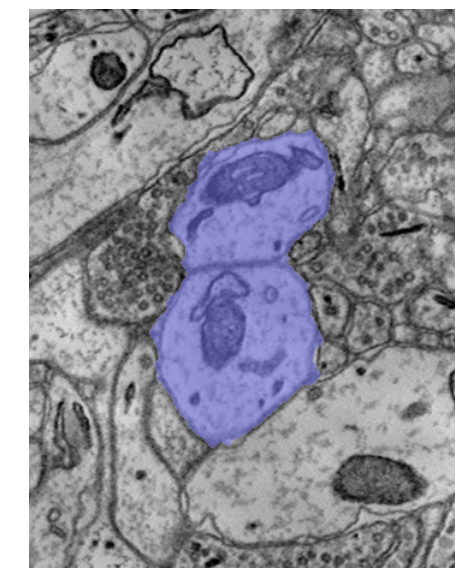
\includegraphics[scale=.22]{gfx/mergeerror.pdf}
\caption{Merge error detection using our classifier: Possible boundaries are generated and rated as split errors using the proposed CNN. The lowest rated boundary which equals the least likely to be a split error is the most likely the correct boundary.}
\label{fig:merge_error}
\end{figure}

Philosophical point of trading split errors for merge errors...


Speed of classification